\section{Results}


\begin{table*}[t]
\centering
\caption{Left: per-category recovery (\%) on Construction problem subsets . Right: robustness to synonym substitution (\% of single-substitution problems solved when the canonical tool is replaced by a synonym). Bold denotes the column-wise maximum.}
\label{tab:combined}
\footnotesize
\renewcommand{\arraystretch}{0.9}
\resizebox{\textwidth}{!}{%
\begin{tabular}{ll|cccccc|cccc}
\toprule
& & \multicolumn{6}{c|}{\textbf{Construction Subsets}} & \multicolumn{4}{c}{\textbf{Synonym Domains}} \\
\midrule
\textbf{Mode} & \textbf{Model} & \textbf{single} & \textbf{chained} & \textbf{bulk} & \makecell{\textbf{stress}\\\textbf{n=10}} & \makecell{\textbf{stress}\\\textbf{n=20}} & \makecell{\textbf{stress}\\\textbf{n=50}} & \textbf{Electronics} & \textbf{Kitchen} & \textbf{Medic} & \textbf{Survival} \\
\midrule
\multirow{3}{*}{\makecell{Consensus\\(n=3)}} & DS & \textbf{100.0} $\pm$ 0.0 & \textbf{100.0} $\pm$ 0.0 & 46.7 $\pm$ 11.5 & \textbf{100.0} $\pm$ 0.0 & \textbf{100.0} $\pm$ 0.0 & \textbf{100.0} $\pm$ 0.0 & \textbf{100.0} $\pm$ 0.0 & 93.3 $\pm$ 20.0 & \textbf{100.0} $\pm$ 0.0 & 95.6 $\pm$ 13.3 \\
 & G4 & \textbf{100.0} $\pm$ 0.0 & \textbf{100.0} $\pm$ 0.0 & \textbf{100.0} $\pm$ 0.0 & \textbf{100.0} $\pm$ 0.0 & \textbf{100.0} $\pm$ 0.0 & \textbf{100.0} $\pm$ 0.0 & \textbf{100.0} $\pm$ 0.0 & 97.8 $\pm$ 6.7 & \textbf{100.0} $\pm$ 0.0 & \textbf{100.0} $\pm$ 0.0 \\
 & G4NT & \textbf{100.0} $\pm$ 0.0 & \textbf{100.0} $\pm$ 0.0 & 46.7 $\pm$ 30.6 & \textbf{100.0} $\pm$ 0.0 & \textbf{100.0} $\pm$ 0.0 & \textbf{100.0} $\pm$ 0.0 & \textbf{100.0} $\pm$ 0.0 & \textbf{100.0} $\pm$ 0.0 & \textbf{100.0} $\pm$ 0.0 & \textbf{100.0} $\pm$ 0.0 \\
\midrule
\multirow{3}{*}{\makecell{Consensus\\(n=5)}} & DS & \textbf{100.0} $\pm$ 0.0 & \textbf{100.0} $\pm$ 0.0 & 86.7 $\pm$ 23.1 & \textbf{100.0} $\pm$ 0.0 & \textbf{100.0} $\pm$ 0.0 & \textbf{100.0} $\pm$ 0.0 & \textbf{100.0} $\pm$ 0.0 & 91.1 $\pm$ 20.3 & \textbf{100.0} $\pm$ 0.0 & \textbf{100.0} $\pm$ 0.0 \\
 & G4 & \textbf{100.0} $\pm$ 0.0 & \textbf{100.0} $\pm$ 0.0 & \textbf{100.0} $\pm$ 0.0 & \textbf{100.0} $\pm$ 0.0 & \textbf{100.0} $\pm$ 0.0 & \textbf{100.0} $\pm$ 0.0 & \textbf{100.0} $\pm$ 0.0 & \textbf{100.0} $\pm$ 0.0 & \textbf{100.0} $\pm$ 0.0 & 97.8 $\pm$ 6.7 \\
 & G4NT & \textbf{100.0} $\pm$ 0.0 & \textbf{100.0} $\pm$ 0.0 & 60.0 $\pm$ 34.6 & \textbf{100.0} $\pm$ 0.0 & \textbf{100.0} $\pm$ 0.0 & \textbf{100.0} $\pm$ 0.0 & \textbf{100.0} $\pm$ 0.0 & \textbf{100.0} $\pm$ 0.0 & \textbf{100.0} $\pm$ 0.0 & \textbf{100.0} $\pm$ 0.0 \\
\midrule
\multirow{3}{*}{Iterative} & DS & \textbf{100.0} $\pm$ 0.0 & \textbf{100.0} $\pm$ 0.0 & 93.3 $\pm$ 11.5 & 93.3 $\pm$ 11.5 & \textbf{100.0} $\pm$ 0.0 & \textbf{100.0} $\pm$ 0.0 & \textbf{100.0} $\pm$ 0.0 & 93.3 $\pm$ 10.0 & \textbf{100.0} $\pm$ 0.0 & \textbf{100.0} $\pm$ 0.0 \\
 & G4 & \textbf{100.0} $\pm$ 0.0 & \textbf{100.0} $\pm$ 0.0 & \textbf{100.0} $\pm$ 0.0 & \textbf{100.0} $\pm$ 0.0 & \textbf{100.0} $\pm$ 0.0 & \textbf{100.0} $\pm$ 0.0 & \textbf{100.0} $\pm$ 0.0 & \textbf{100.0} $\pm$ 0.0 & \textbf{100.0} $\pm$ 0.0 & \textbf{100.0} $\pm$ 0.0 \\
 & G4NT & \textbf{100.0} $\pm$ 0.0 & \textbf{100.0} $\pm$ 0.0 & \textbf{100.0} $\pm$ 0.0 & \textbf{100.0} $\pm$ 0.0 & \textbf{100.0} $\pm$ 0.0 & \textbf{100.0} $\pm$ 0.0 & \textbf{100.0} $\pm$ 0.0 & \textbf{100.0} $\pm$ 0.0 & \textbf{100.0} $\pm$ 0.0 & \textbf{100.0} $\pm$ 0.0 \\
\midrule
\multirow{3}{*}{Judge} & DS & 93.3 $\pm$ 14.1 & 80.0 $\pm$ 20.0 & 26.7 $\pm$ 11.5 & 80.0 $\pm$ 34.6 & 86.7 $\pm$ 11.5 & 86.7 $\pm$ 23.1 & 97.8 $\pm$ 6.7 & 64.4 $\pm$ 41.0 & \textbf{100.0} $\pm$ 0.0 & 93.3 $\pm$ 20.0 \\
 & G4 & 88.9 $\pm$ 22.6 & 93.3 $\pm$ 11.5 & 53.3 $\pm$ 30.6 & 66.7 $\pm$ 41.6 & 80.0 $\pm$ 20.0 & 93.3 $\pm$ 11.5 & \textbf{100.0} $\pm$ 0.0 & 82.2 $\pm$ 25.4 & \textbf{100.0} $\pm$ 0.0 & 97.8 $\pm$ 6.7 \\
 & G4NT & 95.6 $\pm$ 13.3 & \textbf{100.0} $\pm$ 0.0 & 93.3 $\pm$ 11.5 & \textbf{100.0} $\pm$ 0.0 & \textbf{100.0} $\pm$ 0.0 & \textbf{100.0} $\pm$ 0.0 & \textbf{100.0} $\pm$ 0.0 & 93.3 $\pm$ 10.0 & \textbf{100.0} $\pm$ 0.0 & \textbf{100.0} $\pm$ 0.0 \\
\midrule
\multirow{3}{*}{APB} & DS & 55.6 $\pm$ 26.0 & 53.3 $\pm$ 41.6 & 0.0 $\pm$ 0.0 & 53.3 $\pm$ 50.3 & 46.7 $\pm$ 50.3 & 40.0 $\pm$ 20.0 & 64.4 $\pm$ 34.3 & 31.1 $\pm$ 34.8 & 40.0 $\pm$ 26.5 & 44.4 $\pm$ 35.7 \\
 & G4 & 60.0 $\pm$ 43.6 & 80.0 $\pm$ 34.6 & 0.0 $\pm$ 0.0 & 33.3 $\pm$ 57.7 & 46.7 $\pm$ 50.3 & 26.7 $\pm$ 46.2 & \textbf{100.0} $\pm$ 0.0 & 88.9 $\pm$ 33.3 & 95.6 $\pm$ 13.3 & 97.8 $\pm$ 6.7 \\
 & G4NT & 88.9 $\pm$ 33.3 & 33.3 $\pm$ 57.7 & 0.0 $\pm$ 0.0 & \textbf{100.0} $\pm$ 0.0 & \textbf{100.0} $\pm$ 0.0 & 53.3 $\pm$ 50.3 & 57.8 $\pm$ 50.4 & 22.2 $\pm$ 44.1 & 68.9 $\pm$ 47.0 & 88.9 $\pm$ 33.3 \\
\bottomrule
\end{tabular}}
\end{table*}


Table~\ref{tab:macgyver_breakdown} shows the success rate of each experiment configuration across all problem categories. From these experiments we can address \textbf{RQ1}, \textbf{RQ2}, \textbf{RQ3}, and \textbf{RQ5}.

\textbf{RQ1}: across all three presented algorithms, all three LLM model variations are able to generate a solution with a high degree of accuracy. APB is able to generate correct plans, with varying degrees of success.

\textbf{RQ2}: The bulk problems were much harder for the LLM, with APB having a $0\%$ success rate across all models. The LLM typing algorithms are much stronger here, especially the interactive mode of operation wherein Gemma4 both with and without thinking enabled reaching $100\%$ accuracy.

\textbf{RQ5}: Across the different levels of stress configurations, again the interactive algorithm performed the best across all three model variations. APB was able to find successful plans as well  with much lower accuracy.

Nearly across the board, Gemma4 performed better with the LLM typing based approaches, demonstrating at model choice does make a notable difference in performance. The most notable difference between Gemma4 with thinking enabled and without is not performance, which is comparable, but instead with inference time.  

\textbf{RQ6}: Table~\ref{tab:recovery} shows performance across different semantic variations of structural identically PDDL encoding. These different encodings do see fluctuations in accuracy with the interactive approach seeing the highest accuracy across variations. APB is especially effected by this, with the accuracy dropping as low as $46.7\%$ in the medic task with Deepseek. 

\begin{table}
\centering
\caption{Refusal accuracy on unsolvable Construction  problems (\% of runs that correctly fail to produce a plan when no valid substitute exists). APB is omitted because it cannot structurally refuse.} 
\label{tab:refusal}
\footnotesize
\renewcommand{\arraystretch}{0.9}
\begin{tabular}{ll|c}
\toprule
\textbf{Mode} & \textbf{Model} & \textbf{Refusal \%} \\
\midrule
\multirow{3}{*}{\makecell{Consensus\\(n=3)}} & DS & 84.4 $\pm$ 26.0 \\
 & G4 & \textbf{100.0} $\pm$ 0.0 \\
 & G4NT & \textbf{100.0} $\pm$ 0.0 \\
\midrule
\multirow{3}{*}{\makecell{Consensus\\(n=5)}} & DS & 84.4 $\pm$ 24.0 \\
 & G4 & \textbf{100.0} $\pm$ 0.0 \\
 & G4NT & \textbf{100.0} $\pm$ 0.0 \\
\midrule
\multirow{3}{*}{Iterative} & DS & 55.6 $\pm$ 34.3 \\
 & G4 & 24.4 $\pm$ 19.4 \\
 & G4NT & \textbf{100.0} $\pm$ 0.0 \\
\midrule
\multirow{3}{*}{Judge} & DS & 91.1 $\pm$ 10.5 \\
 & G4 & \textbf{100.0} $\pm$ 0.0 \\
 & G4NT & \textbf{100.0} $\pm$ 0.0 \\
\bottomrule
\end{tabular}
\end{table}

\textbf{RQ4}: Table~\ref{tab:refusal} shows the refusal accuracy in problems that do not contain valid solutions. Most configurations show a high refusal percentage, showing that the LLMs will not attempt to make potentially dangerous invalid substitutions. Interestingly, the interactive approach, which performed highly in all other experiments sees a very low accuracy here. This is however, unsurprising as the algorithm continues to loop until a valid plan is found, not allowing the LLM to break the loop. 

Notably, \textsc{Gemma4} without thinking enabled (\textsc{G4NT}) achieves perfect refusal accuracy under the iterative approach, whereas \textsc{Deepseek} and \textsc{Gemma4} with thinking both frequently produce plans for unsolvable problems. Inspection of the results reveals a consistent pattern: thinking-enabled models change objects such as \texttt{ripe-banana} to type \texttt{hammer}, reasoning that its shape makes it a plausible substitute. \textsc{G4NT} is more literal in its type assignments and does not make this leap, correctly leaving such objects as their original type.

\begin{figure}
  \centering
  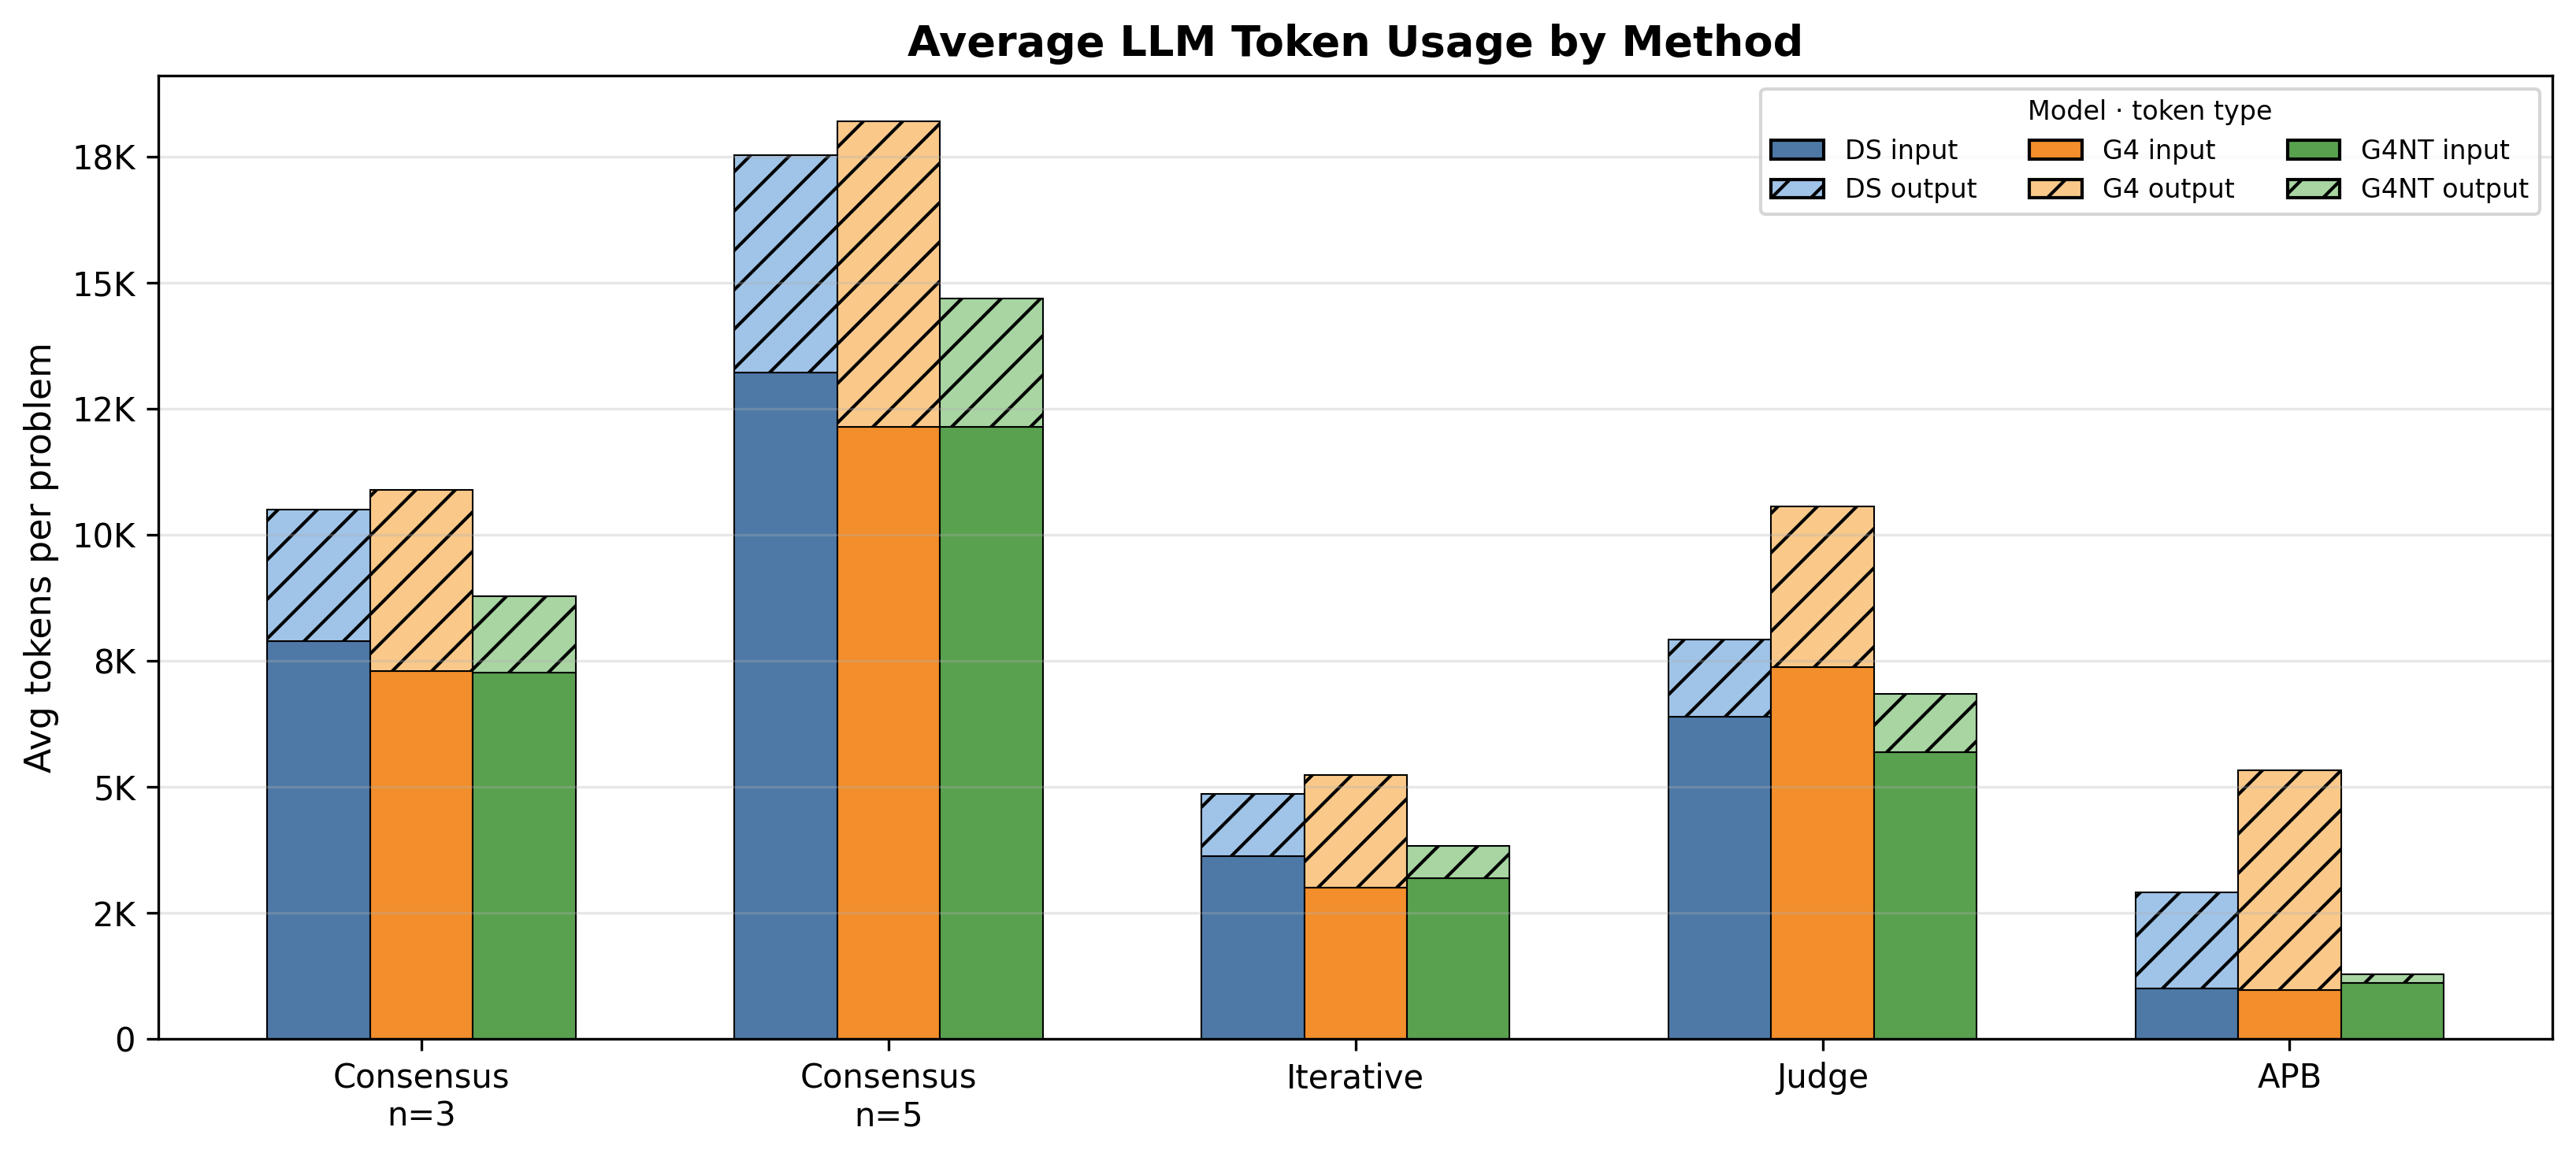
\includegraphics[width=0.45\textwidth]{figures/token_usage.png}
  \caption{\small{Average LLM token usage per problem (input: solid, output: hatched) across methods and models.}}
    \label{fig:token_usage}
\end{figure}

\subsubsection{Token Usage}
Figure~\ref{fig:token_usage} shows average LLM token usage per problem (input and output) across all domains and methods. The consensus methods incur the highest fixed cost, scaling directly with the number of samples: \textsc{n=5} consumes roughly twice the tokens of \textsc{n=3}, as each query is issued independently regardless of outcome. The judge approach falls between the two consensus variants --- it avoids the full \textsc{n=5} sample budget but pays an additional cost for the judge call and any subsequent re-queries when the judge is unsatisfied.

The iterative approach is the cheapest of the typing methods despite its looping behaviour. Unlike consensus, its lower bound is a single LLM query --- a valid plan after the first iteration requires no further calls --- which is reflected in the lower average cost. APB is cheapest overall, though its token profile is notably different: output tokens dominate for thinking-enabled models (\textsc{DS} and \textsc{G4}). \textsc{G4NT}, without a reasoning trace, has the lowest total cost across all methods.
